\section{Experimental Evaluation}
\label{sec:evaluation}

In this section, we evaluate all implemented algorithms extensively and report on the insights gained. For this section, the algorithm from Van Kreveld et al. shall be refered to as the simple algorithm while the Bringmann et al. algorithm shall be refered to as the advanced algorithm. 

\subsection{Data and Hardware}
\label{subsec:hardware}

\subsubsection{Software and Data}
\label{subsubsec:software}

All algorithms were implemented in C++ and compiled using GCC with the O3 flag for compiler optimizations and the flto flag for link time optimizations. The simple algorithms were parallelized using OpenMP with dynamic scheduling and a chunk size of 32 over the two nested for loops iterating over \(i\) and \(j\).

The polylines used in the test cases were automatically generated using a variety of parameters. These include the minimum and maximum allows length for each line segment of the polyline as well as the maximum angle that a line segment is allowed to deviate from the previous one, i.e., a maximum angle of zero degrees can only generate polylines that are effectively straight lines, while a maximum angle of \(180°\) allows for arbitrarily shaped polylines. The reasoning for this is that small angles force the polyline to be more smooth while larger angles cause more erratic and less well-behaved polylines. We test for both well-behaved polylines and non-well-behaved polylines which we define to have a maximum angle of \(60°\) and \(180°\) respectively. 

The minimum and maximum line length are fixed to be \(2\) and \(10\). The exact values for the maximum line length is arbitrary as any polyline can be scaled accordingly and achieve the same results by scaling the respective \(\varepsilon\) value. The minimum line segment length of \(2\) was enforced for three primary reasons: 
\begin{itemize}
	\item To prevent the simulation of arbitrary angles through chains of infinitesimally short line segments.
	\item To reduce the variance in line segment lengths, improving the clarity of visualizations.
	\item To mitigate numerical instability and avoid divisions by zero that could occur with zero-length segments, which our algorithms do not explicitly handle.
\end{itemize}

To generate the polylines, we fix the first point of the polylines to be the origin (remember that the simplifications are invariant under translation) and following that we sample an initial angle arbitrarily uniformly distributed. This does not use the maximal angle yet. Following that we iteratively sample a line segment length and an angle which is added to the current total angle. Using these two values the next point of the polylines is generated. Each angle is chosen uniformly distributed in the range \([-\alpha, \alpha]\) where \(\alpha\) is the maximum angle as explained before. The line segment length is not chosen uniformly as we want to sample the next point uniformly from the annular sector defined by the maximal angle and the line lengths. To achieve this we use inverse transform sampling resuling in choosing the line segment lengths as \(\sqrt[d]{m^d + (M^d-m^d)U}\) where \(d\) is the dimension, \(m\) and \(M\) are the minimum and maximum line segment length respectively and \(U\) is a uniform distribution on \([0,1]\). This generation principle should work in arbitrary dimensions but we restrict ourselves to two dimensions as that is the most relevant use case and can be visualized well.

Examples of such generated polylines can be seen in \cref{fig:well-behaved-300} and \cref{fig:non-well-behaved-300}.

\begin{figure}[b]
  \centering
  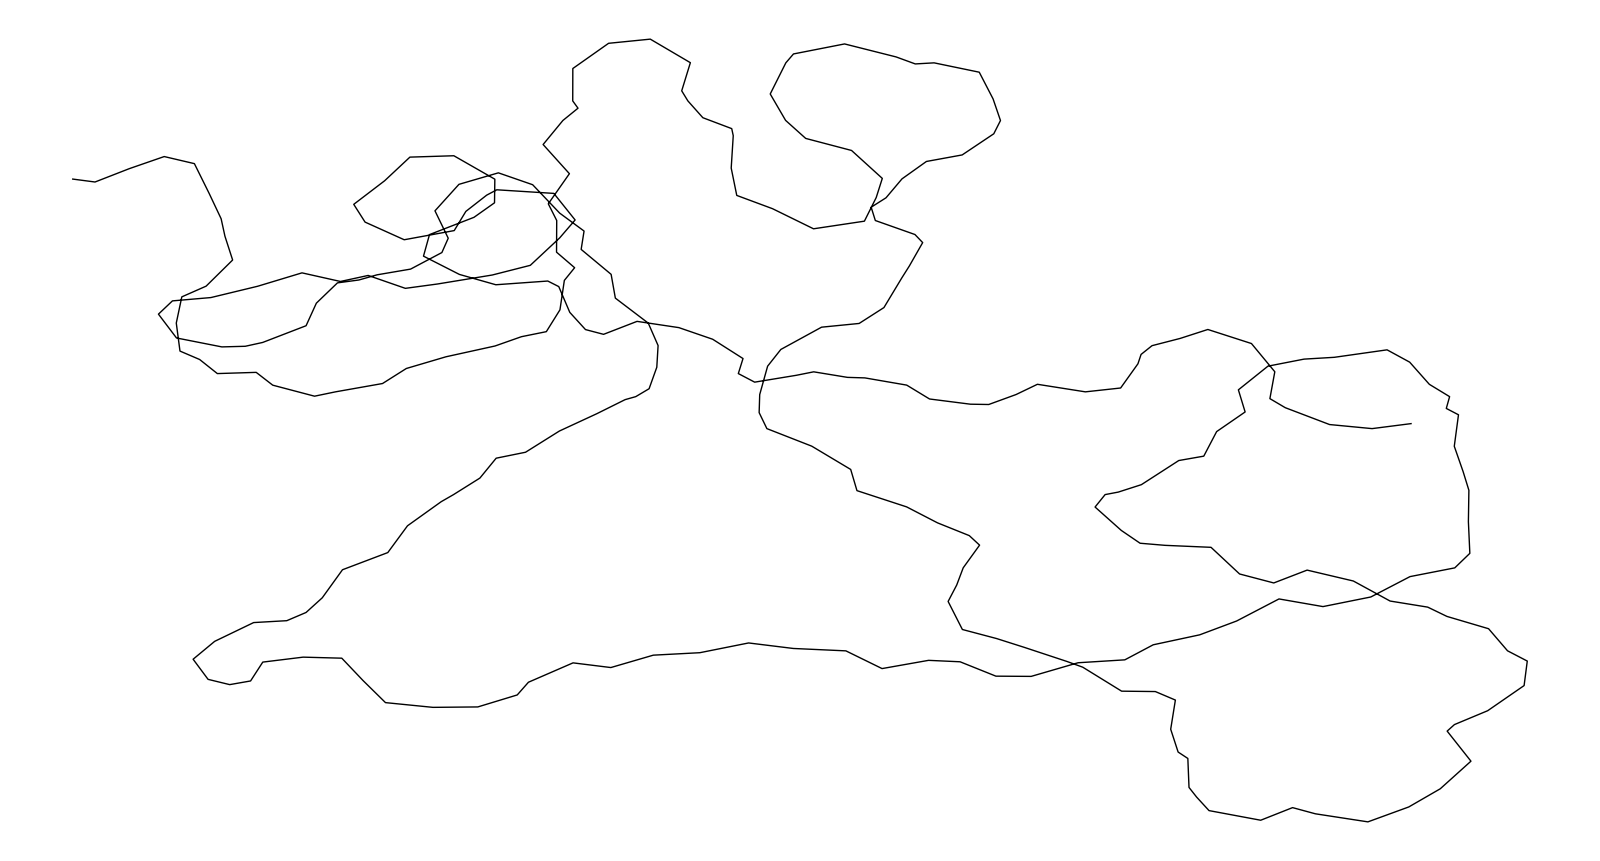
\includegraphics[scale=0.3]{./figures/well-behaved-300.png}
  \caption{Example of a well-behaved polyline consisting of \(300\) points in \(2\) dimensions.}
  \label{fig:well-behaved-300}
\end{figure}

\begin{figure}[b]
  \centering
	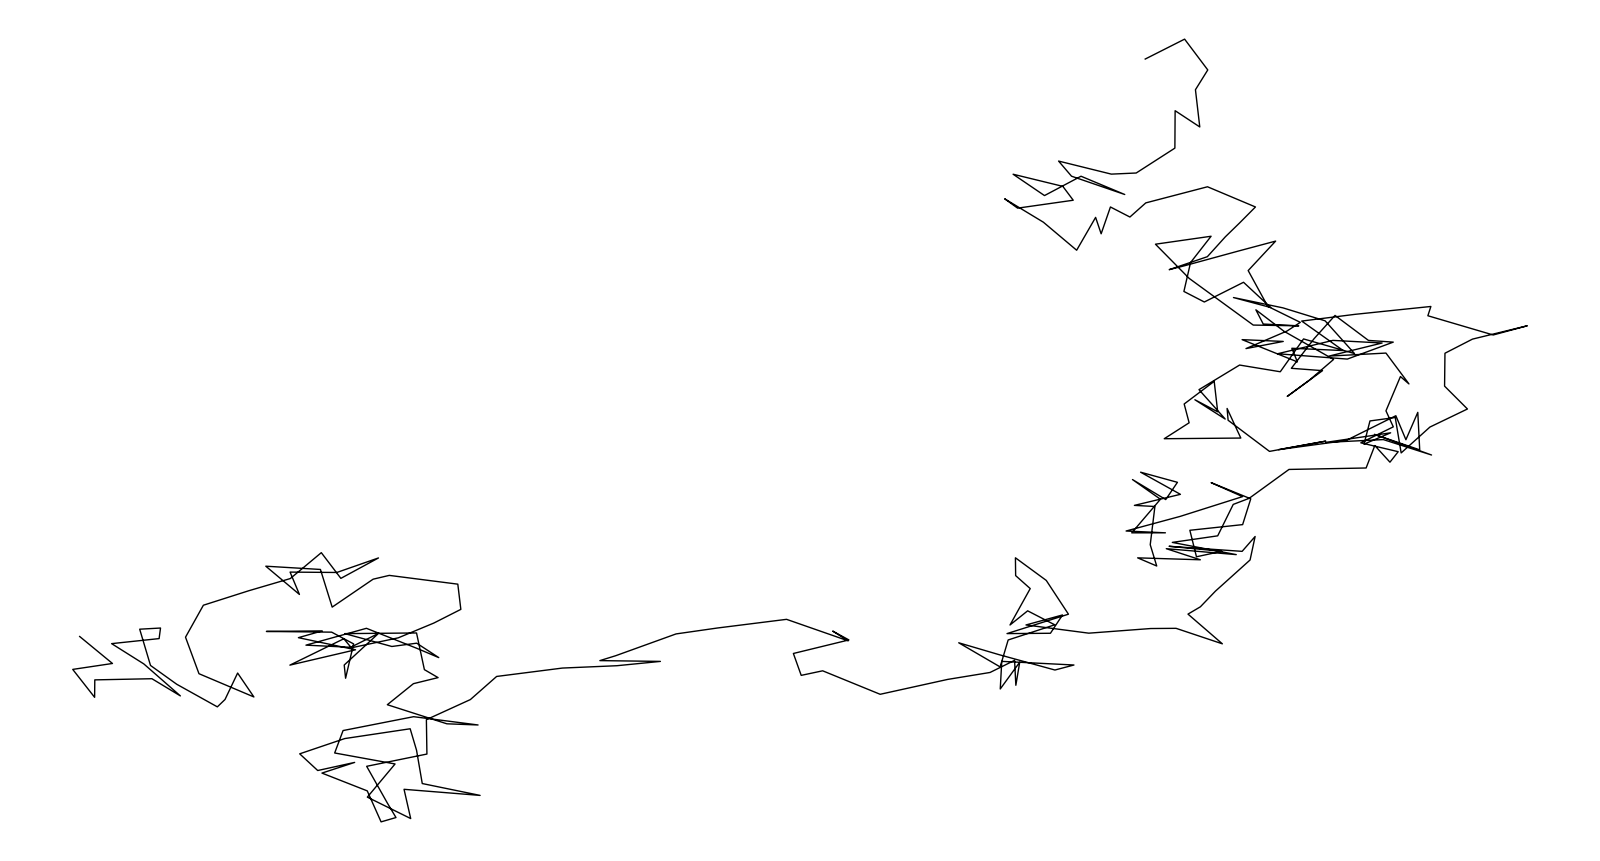
\includegraphics[scale=0.3]{./figures/non-well-behaved-300.png}
  \caption{Example of a non-well-behaved polyline consisting of \(300\) points in \(2\) dimensions.}
  \label{fig:non-well-behaved-300}
\end{figure}

\subsubsection{Hardware}
\label{subsubsec:hardware}
The experiments were conducted on a system with an AMD Ryzen 5 7520U CPU (4.38 GHz, 8 cores) running Arch Linux.

\subsection{Experimental Setup}
\label{subsec:exp_setup}

We test the following nine variants:
\begin{itemize}
	\item Simple Euclidean Algorithm 
	\item Simple Manhattan Algorithm 
	\item Simple Chebyshev Algorithm 
	\item Simple Implicit Euclidean Algorithm 
	\item Simple Semiexplicit Euclidean Algorithm 
	\item Advanced Euclidean Algorithm 
	\item Advanced Manhattan Algorithm 
	\item Advanced Chebyshev Algorithm 
	\item Advanced Semiexplicit Euclidean Algorithm 
\end{itemize}

We have not implemented an implicit version of the advanced algorithm as it would require a complete rewrite of the complicated Bringmann et al. algorithm as well as all of its dependencies. All non-implicit variants (including the semiexplicit ones) on the other hand can be implemented as a single algorithm where the necessary changes can be abstracted in a C++ template to reduce code duplication. 

Due to the extensive parameter space and potential variations that can be tested, a comprehensive evaluation of every possibility is infeasible. We thus must select which criteria to test and which are fixed. We encourage the interested reader to try different variations as we observed that even minor changes may lead to different results. 

Notably, during preliminary testing, five of the nine main algorithms proved to be the fastest under different conditions (e.g., compiler flags, input size), highlighting the high dependency of performance on the experimental environment. The specific variants were:
\begin{itemize}
	\item Simple Implicit Euclidean in a concurrent setting on small polylines 
	\item Simple Chebyshev under parallel execution without link time optimization on small polylines 
	\item Advanced Chebyshev without link time optimization on long polylines 
	\item Simple Euclidean under parallel execution with link time optimization on small polylines 
	\item Advanced Euclidean with link time optimization on long polylines 
\end{itemize}
Note that this does not mean that those conditions were the optimal conditions for the individual algorithms but instead reflects their speed relative to the other variants.

We have already mentioned some of our choices but for completeness we list all of them, not only the ones that have not been mentioned yet. Many of the effects on the runtime may be implementation, hardware or even operating system specific thus we cannot guarantee the same effects. 

\begin{itemize}
  \item Compiler optimizations with the O3 flag: This generally resulted in a performance boost of a factor of \(10\) on all variants and there was no reason to test the algorithms without optimizations.
	\item Link time optimizations with the flto flag: For most variants enabling this flag resulted in a \(20\%\) performance boost. The only exception being the semiexplicit version of the simple algorithm which for unknown reasons is noticeably slower.
	\item Parallelization of the simple algorithms using eight cores: This speeds up the implicit and semiexplicit versions by about three times and the explicit ones by six to seven times. The difference can be attributed to the more complicated comparisons in the non-explicit versions which may lead to worse parallelizability. 
	\item Well-behaved and non-well-behaved polylines: We test on both types of polylines where well behaved ones have a maximum angle of \(60^\circ\) and non-well-behaved ones have a maximum angle of \(180^\circ\). The lengths of the lines segments are restricted to be within \([2, 10]\). 
	\item Choice of \(\varepsilon\): We generally choose \(\varepsilon = 2\) if not stated otherwise. The reason for this is a technical one, namely it has the property that \(\varepsilon^2 \neq \varepsilon\) which we wanted to be able to notice mistakes in the semiexplicit implementations more easily as those use \(\varepsilon^2\) instead but must yield the same result as the explicit version. This has no effect on the runtime of the advanced algorithms but together with the data generation, this naturally affects the size of the simplifications and thus the runtime of the simple algorithms.
	\item Many implementation details affect the runtime more than expected. For example, we observed that inlining some functions can speed up or slow down some algorithms by upto \(20\%\). We tried to choose the versions with the best performance but it is likely that some better choices exist depending on compiler and hardware. 
\end{itemize}

\subsection{Optimization Tests}
Before we present the actual results, we explore the effects of the optimizations from \cref{ssec:optimizations} applied on the simple algorithm. In the following section, we will use all optimizations for further comparisons.

We have the following optimizations to test:
\begin{itemize}
	\item Parallelization (p)
	\item Reachability optimization (r)
	\item Local minimality optimization (l)
	\item Global minimality optimization (g)
\end{itemize}

For the parallelized setting we compare fully parallelized with \(8\) cores against no parallelization. For the other three we test having the optimization and not having them. Further, we test the algorithm with no optimizations applied. All of these tests are on well-behaved data and \(20\) cases per point count on polylines upto length \(200\).

First, we compare the effect of parallelization. \cref{fig:simple-seq} shows both the unparallelized and the parallelized versions. The parallelized versions are consistently about three times faster than the unparallelized ones.

\begin{figure}[b]
  \centering
	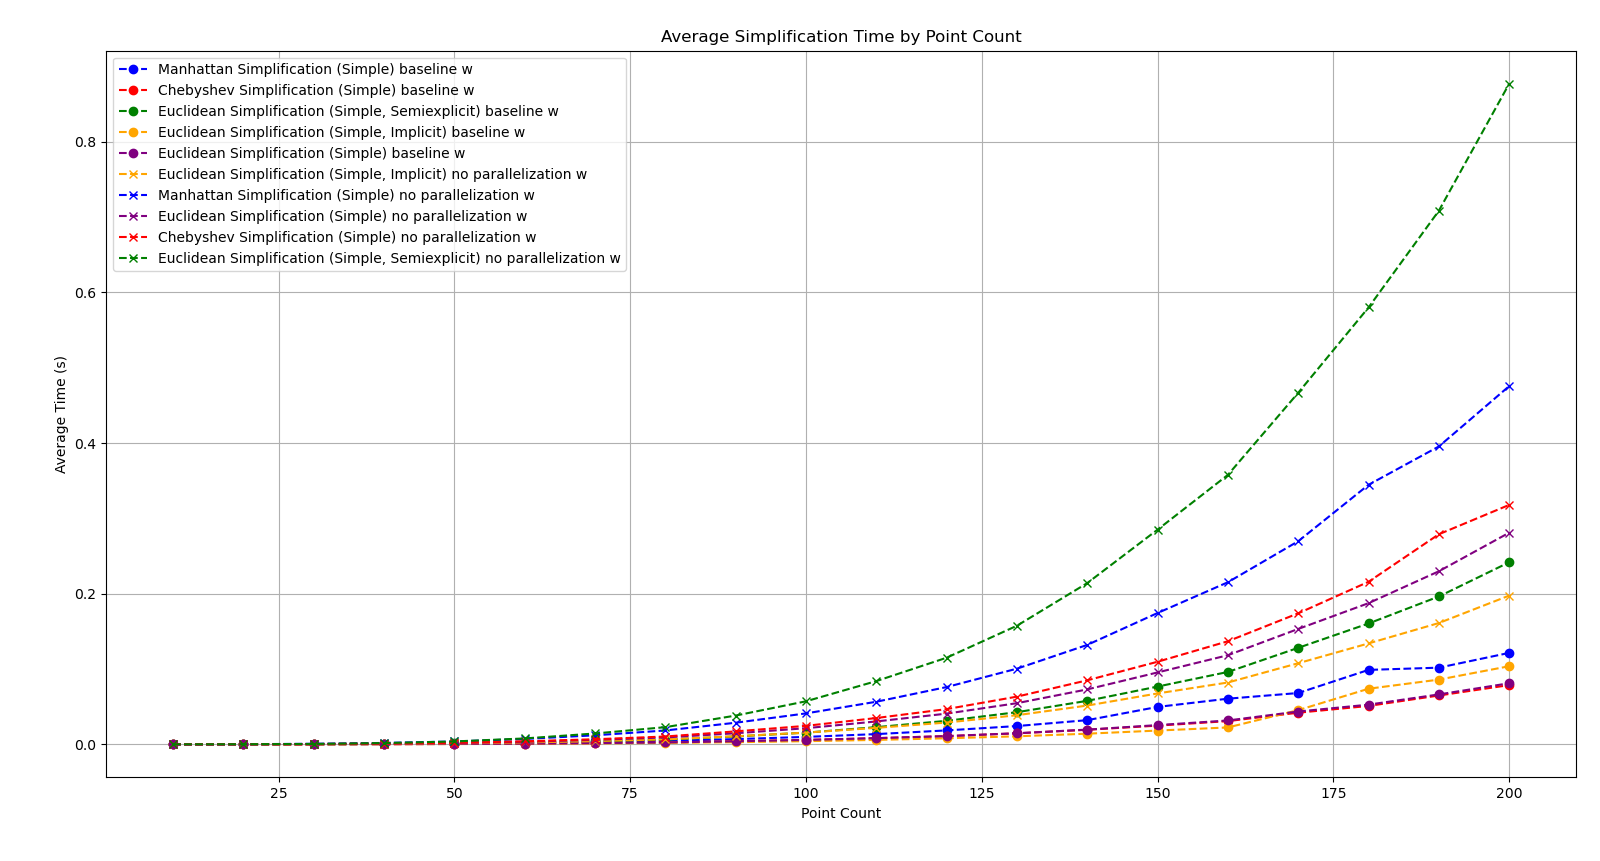
\includegraphics[scale=0.4]{./figures/simple-seq.png}
  \caption{Simple algorithm with and without parallelization}
  \label{fig:simple-seq}
\end{figure}

Next, we inspect how our optimizations affect the runtime. All of the following are parallelized. \cref{fig:simple-noopt} compares having all three optimizations and none of them. Without any of them, the theoretical \(\Oh(n^6)\) runtime seems to match. It further illustrates how effective these small optimizations are.

\begin{figure}[b]
  \centering
	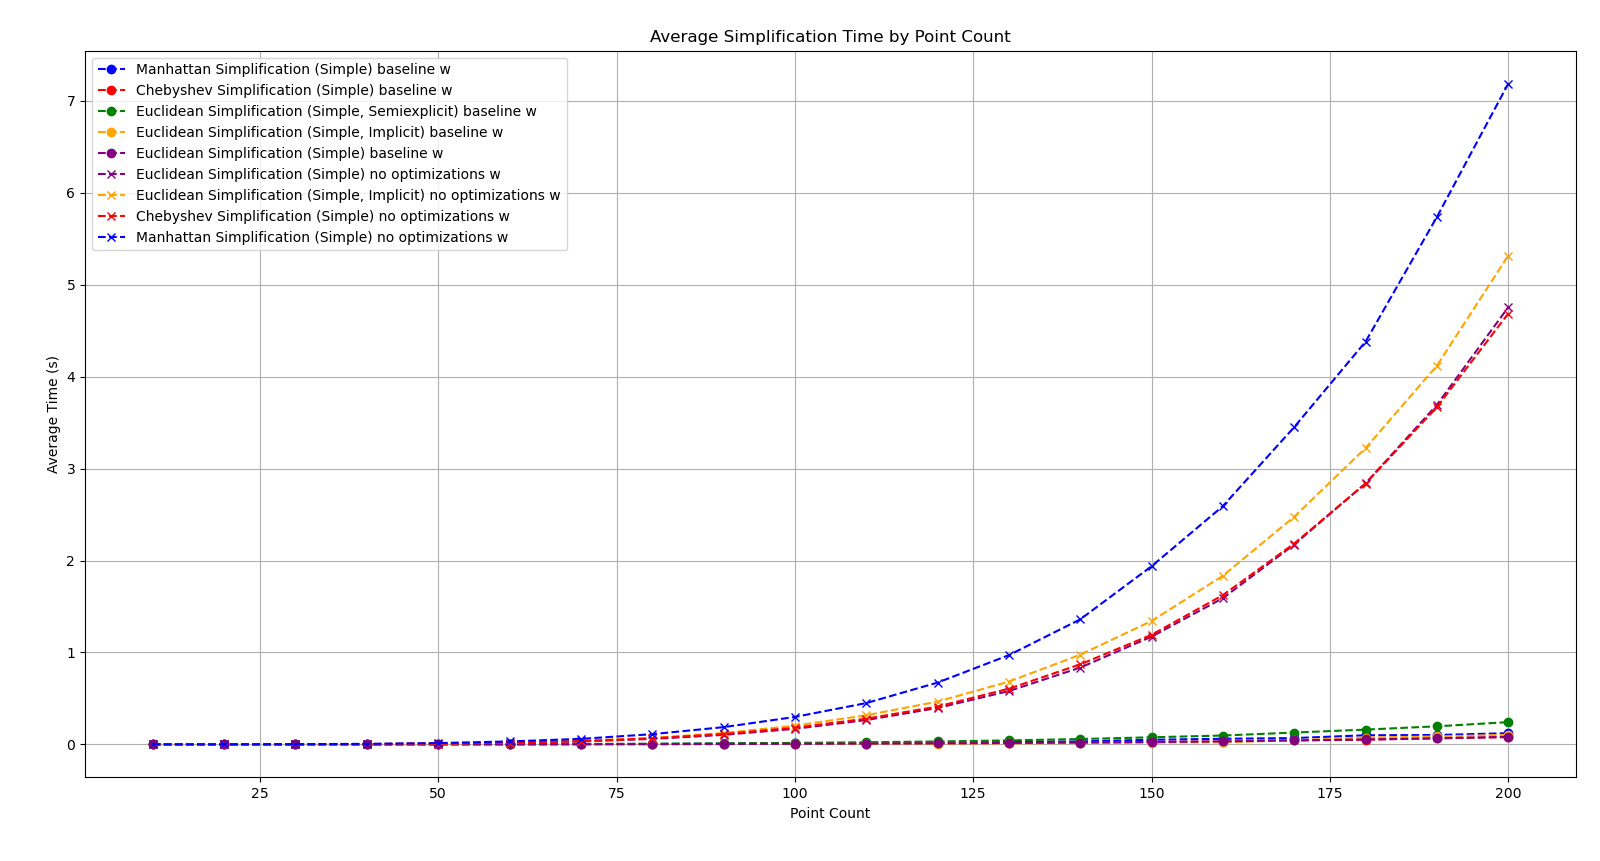
\includegraphics[scale=0.4]{./figures/simple-noopt.png}
  \caption{Simple algorithm with all optimizations and with none of them.}
  \label{fig:simple-noopt}
\end{figure}

Finally, we compare omitting exactly one of the three optimizations. \cref{fig:simple-g} does not have the global optimality optimization, \cref{fig:simple-l} lacks the local optimality optimization, and \cref{fig:simple-r} does not use the reachability optimization. 

The reachability optimization has little effect on most variants but a massive one on the implicit variant. We have no good reasoning why that is the case whereas the other variants are mostly unaffected as the main logic should be the same for all variants.

The local minimality optimization also has almost no effect on most variants with the noticeable outlier again being the implicit variant as well as a slight but consistent improvement in the Manhattan variant.

The global minimality optimization has the most positive effect. We note again that \cref{fig:simple-g}, \cref{fig:simple-l}, and \cref{fig:simple-r} have two of the optimizations but omit one of them. It is noticeable that the performance improvements from these three diagrams does not add up to the performance difference seen in \cref{fig:simple-noopt} which suggests that all these optimizations have a large overlap in what parts of the algorithm they speed up. This can especially be explained in the local and global minimality optimizations: If the local one is triggered in any layer of the algorithm, the global version will be triggered in all following layers for the same cell entry. This explains why the global minimality seems to be better. 

In the actual results we use all optimizations and parallelization for the tests as they have proven to be beneficial, especially for the implicit variant. 

\begin{figure}[b]
  \centering
	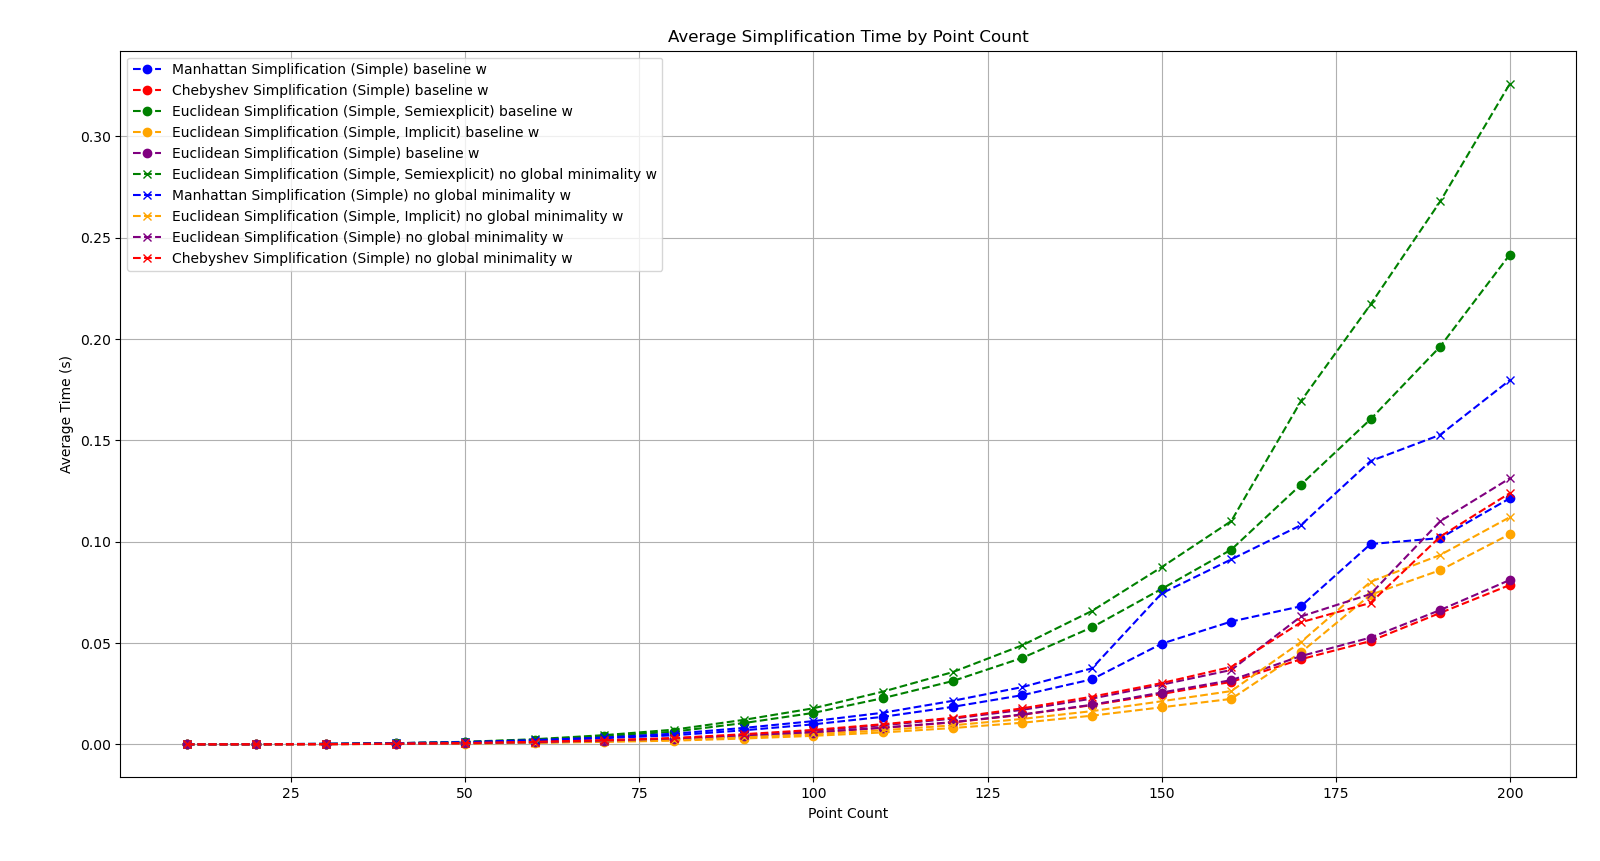
\includegraphics[scale=0.4]{./figures/simple-g.png}
  \caption{Simple algorithm with all optimizations and with all but the global optimality optimization.}
  \label{fig:simple-g}
\end{figure}

\begin{figure}[b]
  \centering
	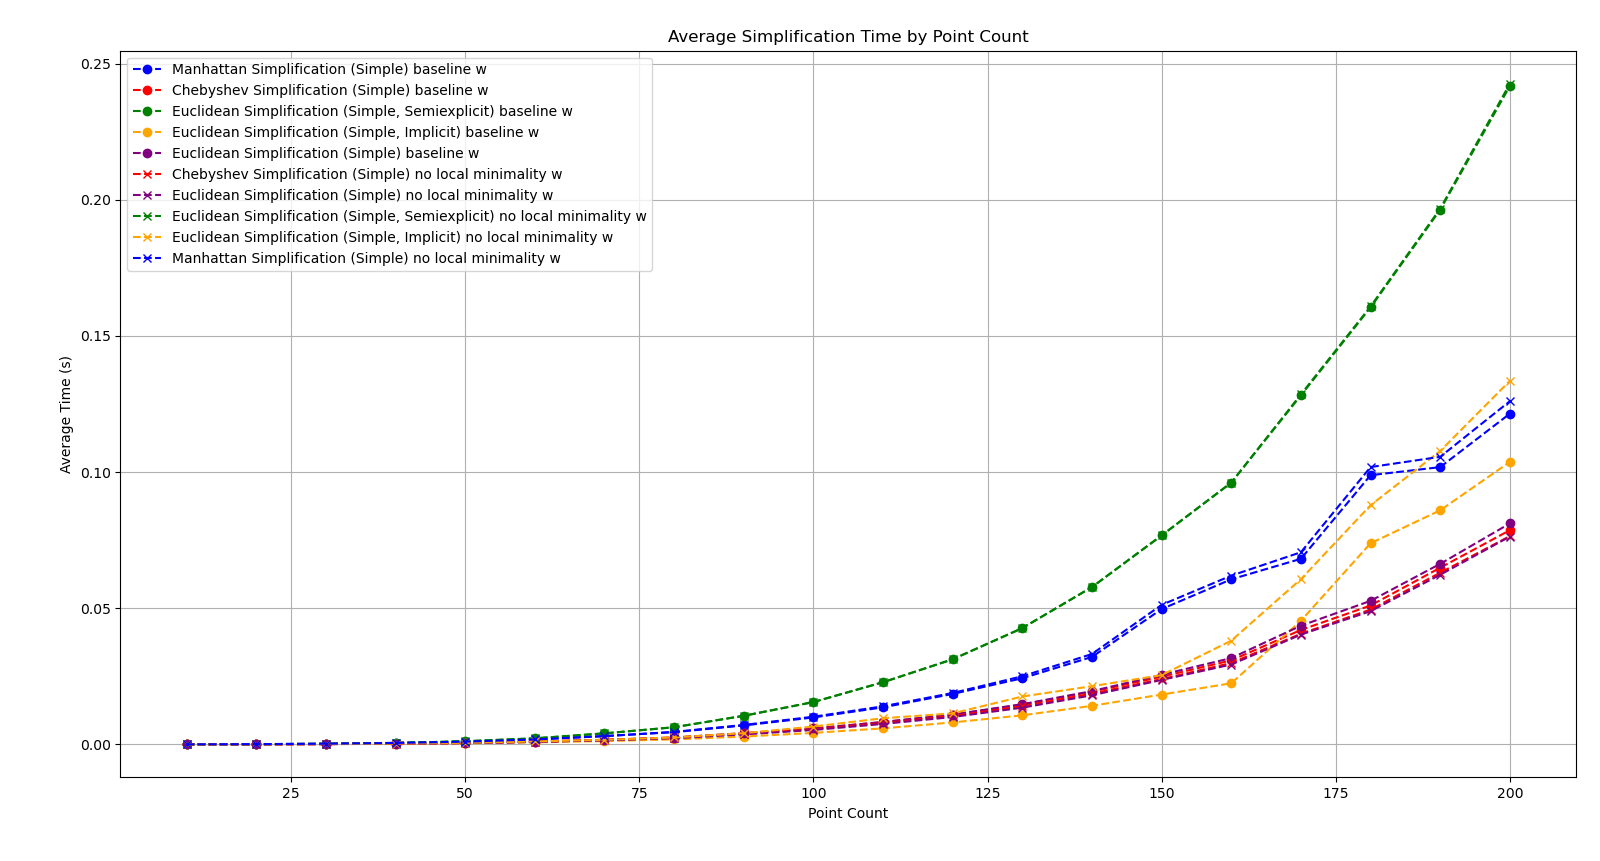
\includegraphics[scale=0.4]{./figures/simple-l.png}
  \caption{Simple algorithm with all optimizations and with all but the local optimality optimization.}
  \label{fig:simple-l}
\end{figure}

\begin{figure}[b]
  \centering
	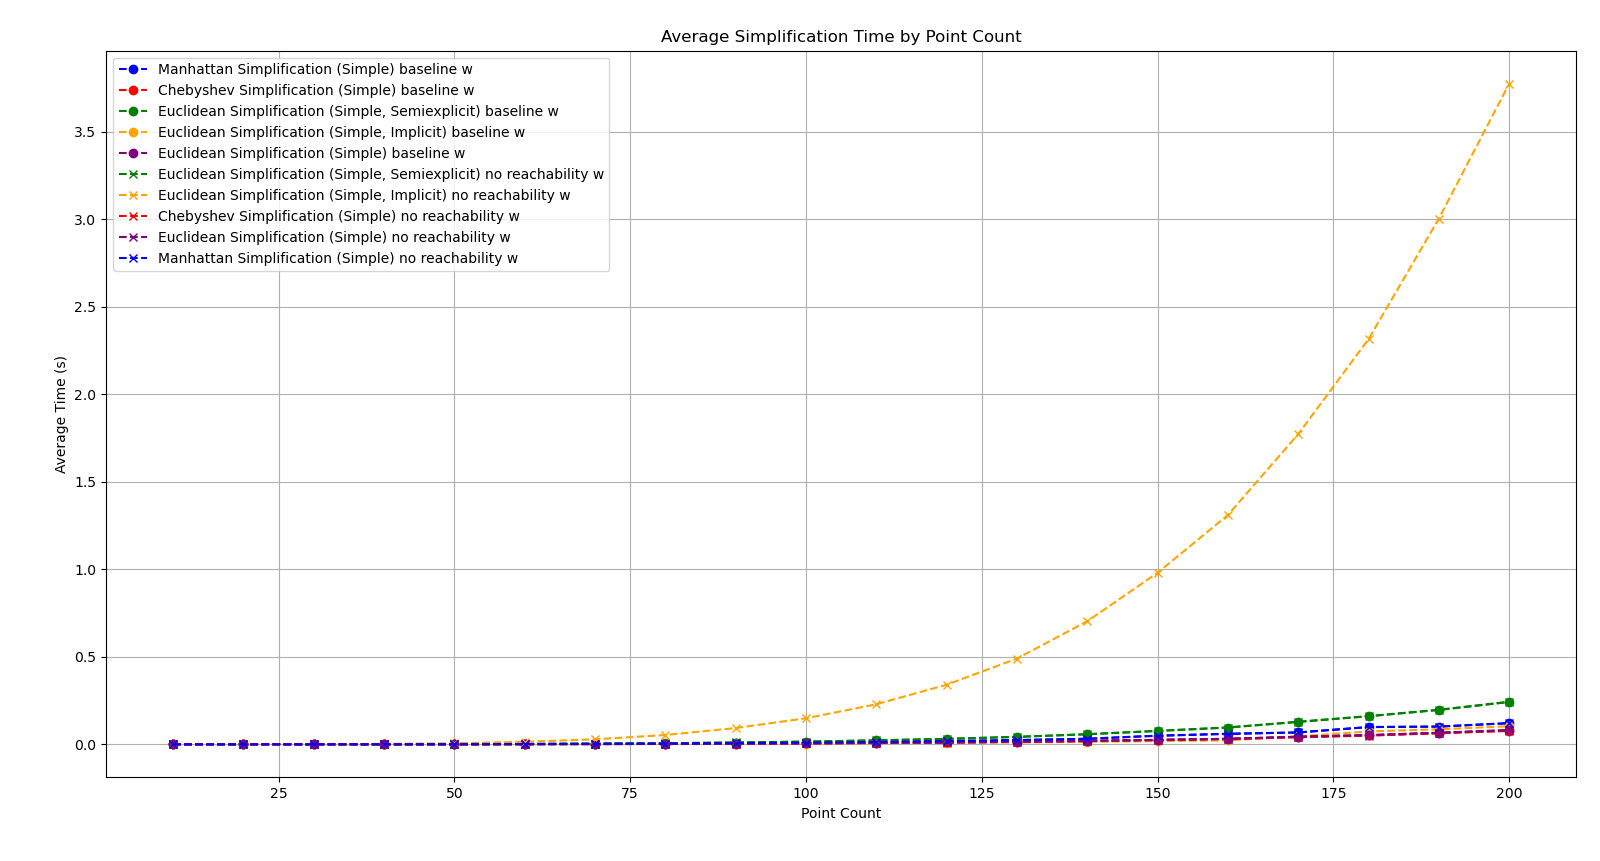
\includegraphics[scale=0.4]{./figures/simple-r.png}
  \caption{Simple algorithm with all optimizations and with all but the reachability optimization.}
  \label{fig:simple-r}
\end{figure}

\subsection{Results}
\label{subsec:results}

We present the results of our experimental evaluation, structured into two parts. First, \cref{ssubsec:runtime}, we perform a comprehensive analysis  of the runtime performance of all nine algorithm variants. Second, in \cref{ssubsec:simplification_size}, we evaluate the quality of the simplifications by comparing their outputs. 

\subsubsection{Runtime}
\label{ssubsec:runtime}

\cref{fig:res_all300w} shows a first overview over all nine variants on well-behaved data. The advanced versions are faster on longer polylines while the simple variants stay competetive due to parallelization and utilizing the well-behavedness of the input data. The semiexplicit Euclidean and Manhattan variants are in both simple and advanced algorithms the slowest. For the simple variant the semiexplicit version is by far the slowest which we think is because of worse parallelizability that is caused by the more complicated comparison operator. For the advanced versions, Manhattan becomes the slowest variant. We think that is because it has the most complicated equation solving algorithm out of all variants and cannot use better parallelization to beat the semiexplicit variant.

\begin{figure}[b]
  \centering
	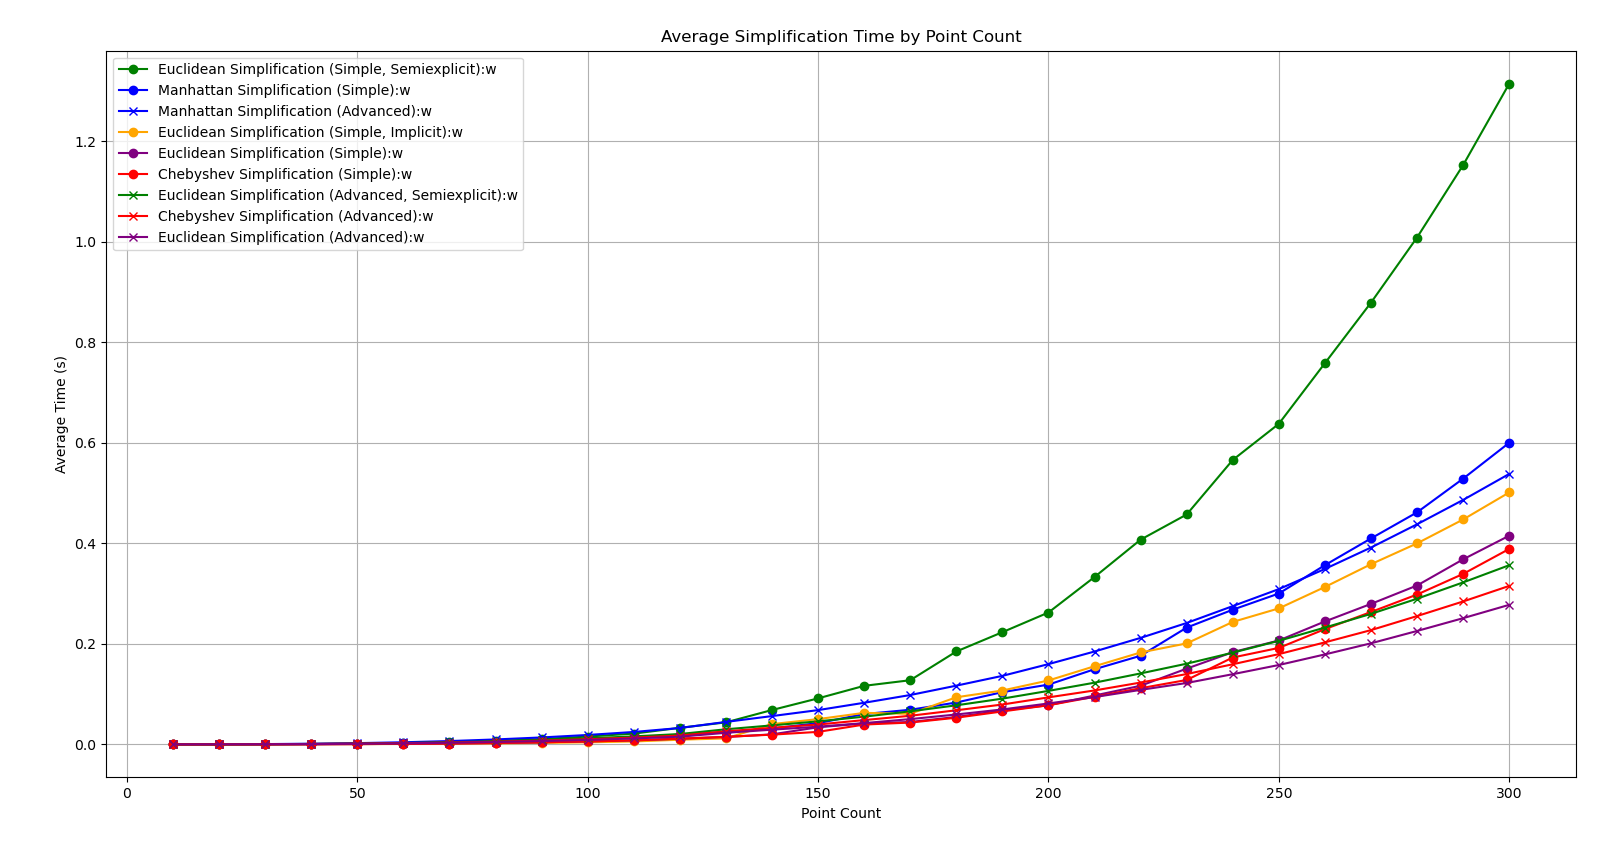
\includegraphics[scale=0.4]{figures/res_all300w.png}
  \caption{All nine variants on well-behaved data. Measurements are averages over 30 polylines per point count. Data that is marked with an ``x" are the advanced variants, those marked with dots are the simple variants. }
  \label{fig:res_all300w}
\end{figure}

It may be notable that we were even able to perform experiments on polylines of that size given the bad theoretical runtimes of \(\O(n^3)\) and \(\O(n^6)\) respectively\footnote{As can be seen in \cref{ssubsec:simplification_size} the output sizes scale approximately linear on the tested polylines thus the runtime of the simple algorithm is closer to \(\O(n^6)\) than \(\O(n^5)\).}. This can be explained as the individual operations are simple artihmetical operations that can be performed fast on modern hardware.

Further, it is remarkable how smooth the data for the advanced variants is. The Bringmann et al. algorithm always performs the same computations regardless of the input polyline but this degree of stability is surprising. 

We extend the evaluation of the advanced variants to polylines of upto 800 points to further get insights on how they scale. As we have already seen they are remarkably stable so we reduced the test cases per polyline length to \(2\) to reduce the total testing time. The results can be seen in \cref{fig:res_advanced800} and even though there is now more variance in the individual data points the trend is undeniably stable and without further surprises. It can also be seen that these variants are insensitive to the well-behavedness of the data which was expected. 

\begin{figure}[b]
  \centering
	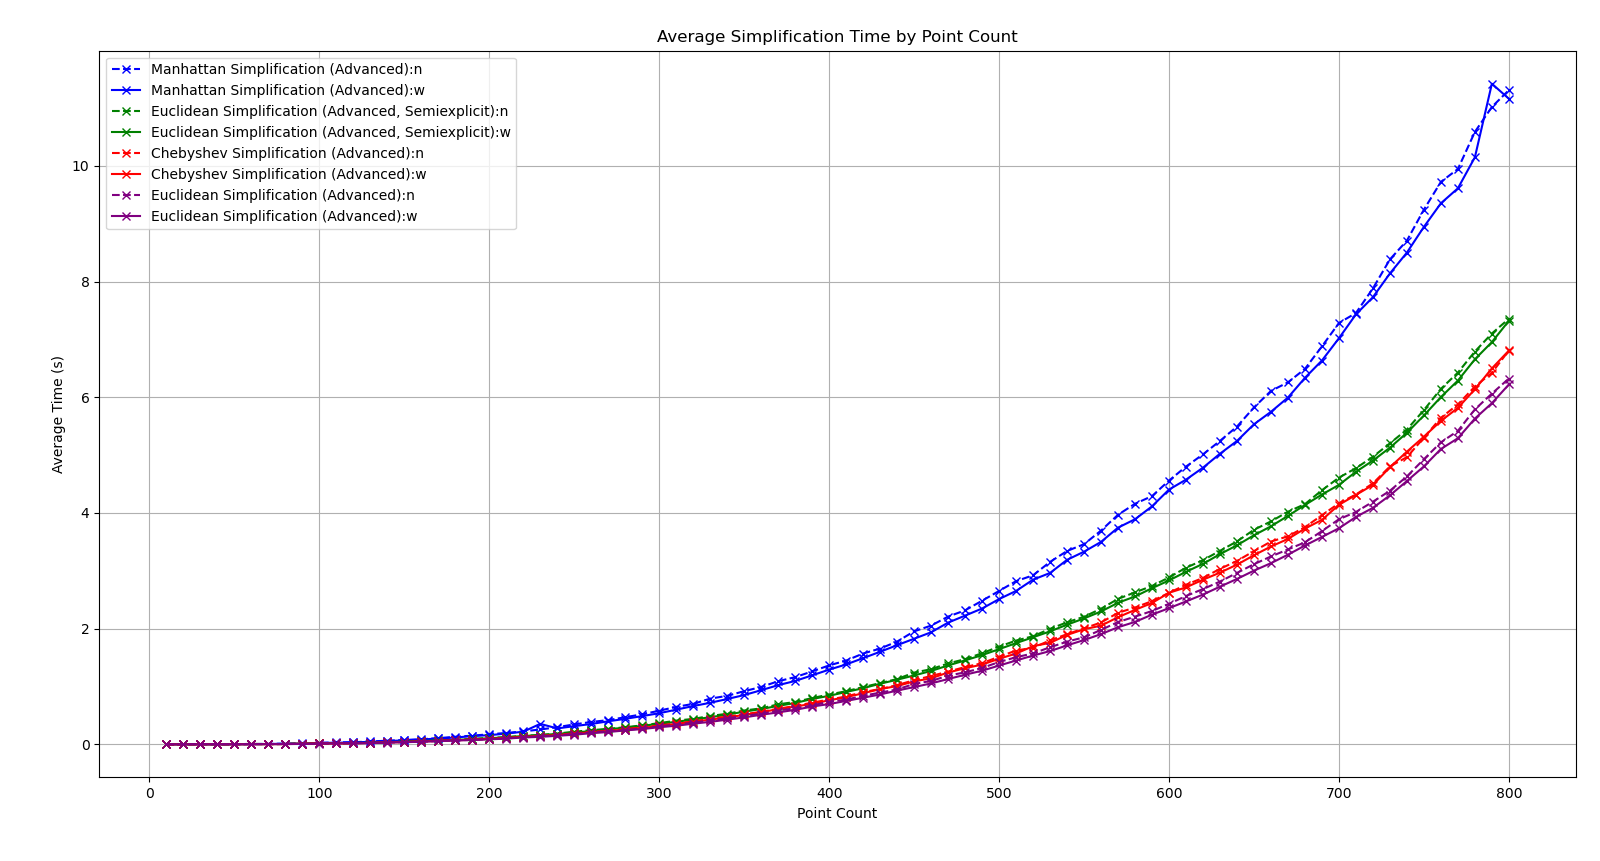
\includegraphics[scale=0.4]{./figures/res_advanced800.png}
  \caption{All advanced variants on well-behaved data and non-well-behaved data. This uses only two cases per polyline size.}
  \label{fig:res_advanced800}
\end{figure}

At this point, we note that the reason that we did not test longer polylines was that during preliminary testing we observed that polylines of length 1000 would use too much memory and thus terminate while ones with 800 points still worked. We did not test what the exact boundary is because it is implementation and hardware dependent and we wanted to perform the tests with enough memory that all of them would execute without problems. 

We now examine in more detail the dependence of the input data on the runtime of the simple algorithm in \cref{fig:res_simple}. If we ignore the semiexplicit variant (which are the slowest variants), all variants on well-behaved polylines take less time than any variant on non-well-behaved data. Another interesting insight is that the runtimes are more consistent on well-behaved data while there is more variance in the non-well-behaved data. 

\begin{figure}[b]
  \centering
	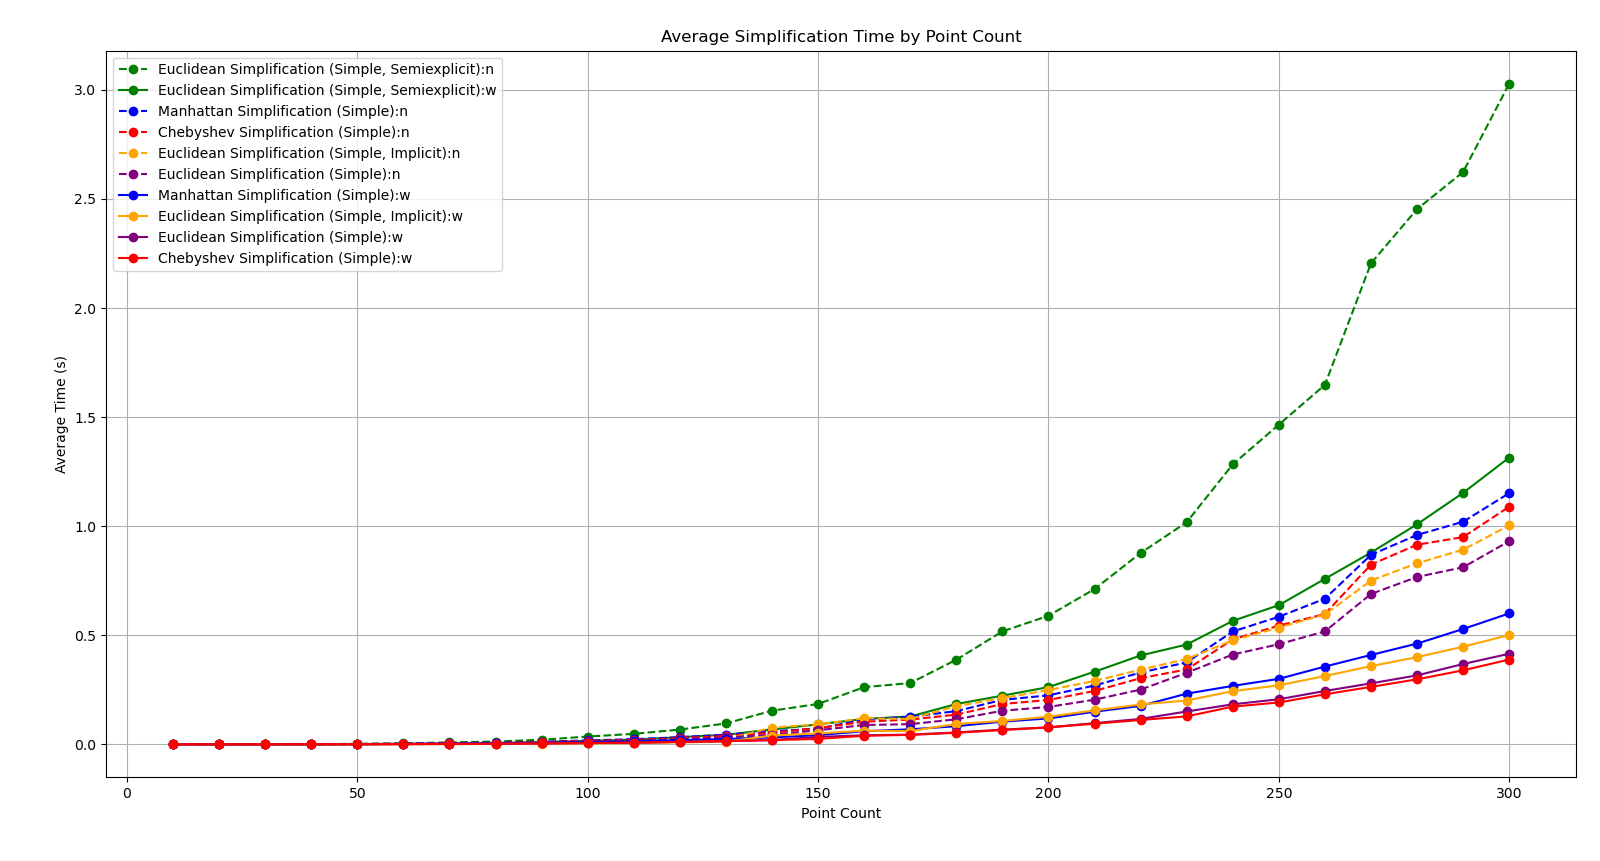
\includegraphics[scale=0.4]{./figures/res_simple.png}
  \caption{Effect of well-behavedness on the runtime of the simple algorithms.}
  \label{fig:res_simple}
\end{figure}


Finally, we can see the runtime of \cref{algo:query-datastructure} in \cref{fig:res_ds}. We only used one test case per point count not only for shorter testing times but to highlight the stability of this algorithm. This very noticable stability of the runtime can be explained by the already seen stability of the advanced algorithm that is used and the predictable amount of simplifications that need to be performed due to the binary search.

\begin{figure}[b]
  \centering
	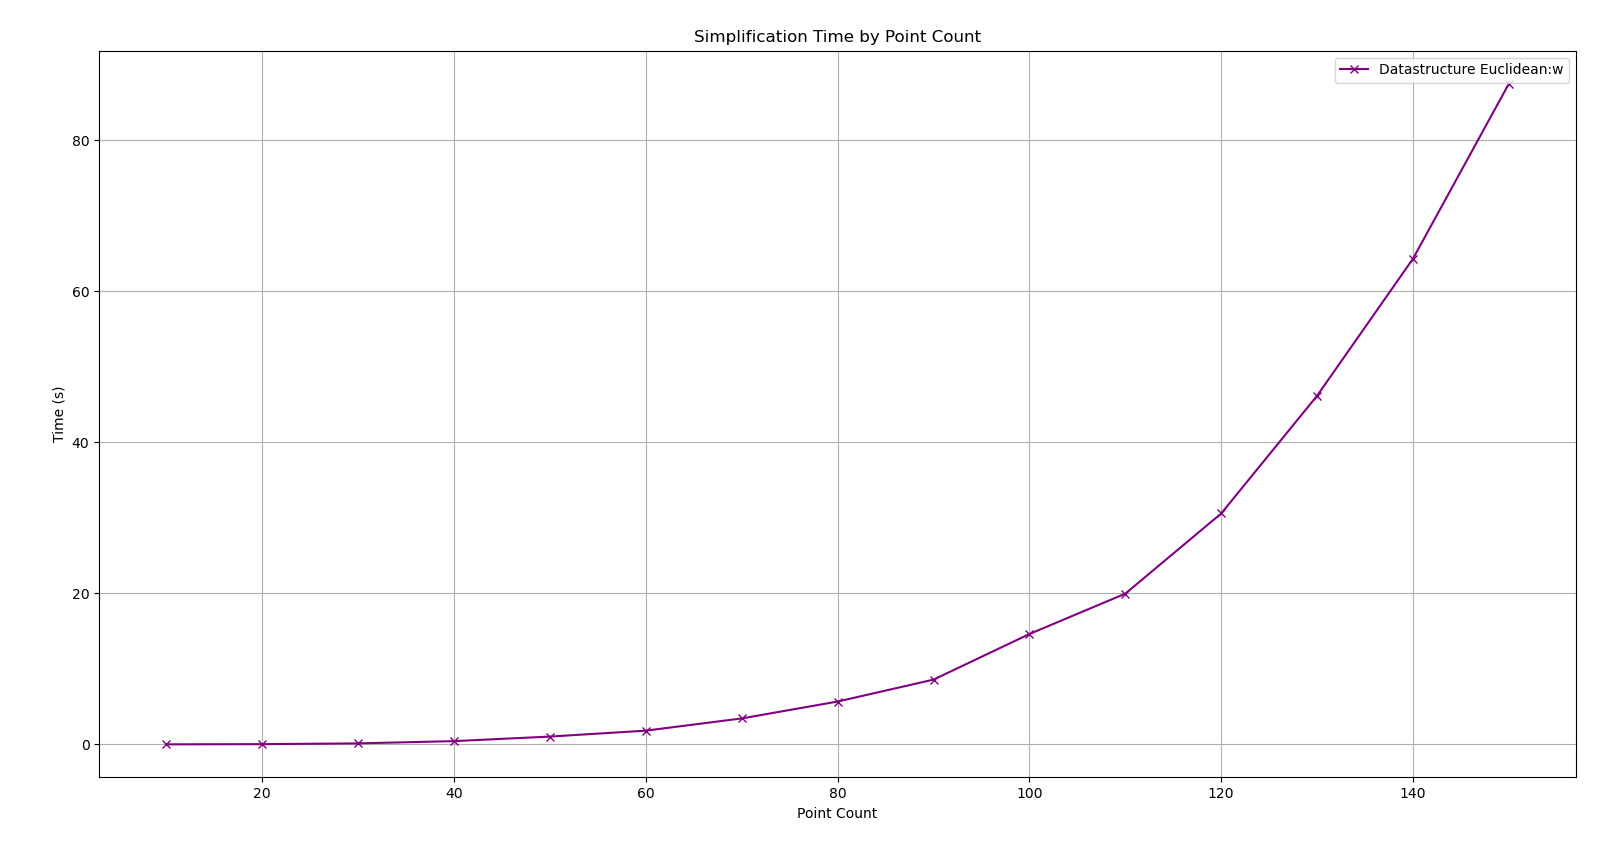
\includegraphics[scale=0.4]{./figures/res_ds.png}
  \caption{Runtime to create the datastructure to query for simplifications using Euclidean distance and one case per point count.}
  \label{fig:res_ds}
\end{figure}


\subsubsection{Simplification Size}
\label{ssubsec:simplification_size}
Having compared the performance of the algorithms, we now compare the simplifications and their sizes. This is independent of the algorithm used but instead only depends on the distance type, input data, and the epsilon used.

\cref{fig:simplification_sizes} shows the averaged computed sizes of the same data that was used for \cref{fig:res_all300w} and \cref{fig:res_simple}. It can clearly be seen that the Chebyshev simplifications are the smallest and the Manhattan ones are the largest which we already know from \cref{cor:size_monotonicity}. However, the sizes are more impacted by the well-behavedness than by the distance used as the difference between the well-behaved Manhattan and the non-well-behaved Chebyshev simplifications is larger than the difference between the non-well-behaved or the well-behaved respectively. Other Minkowski distances \(\delta_\ell\) would fall in the region between the Euclidean and Chebyshev distance if \(\ell > 2\) or between the Euclidean and Manhattan distance if \(\ell \in (1,2)\) so there would not be more spread in those well-behavednes clusters.

\begin{figure}[b]
  \centering
	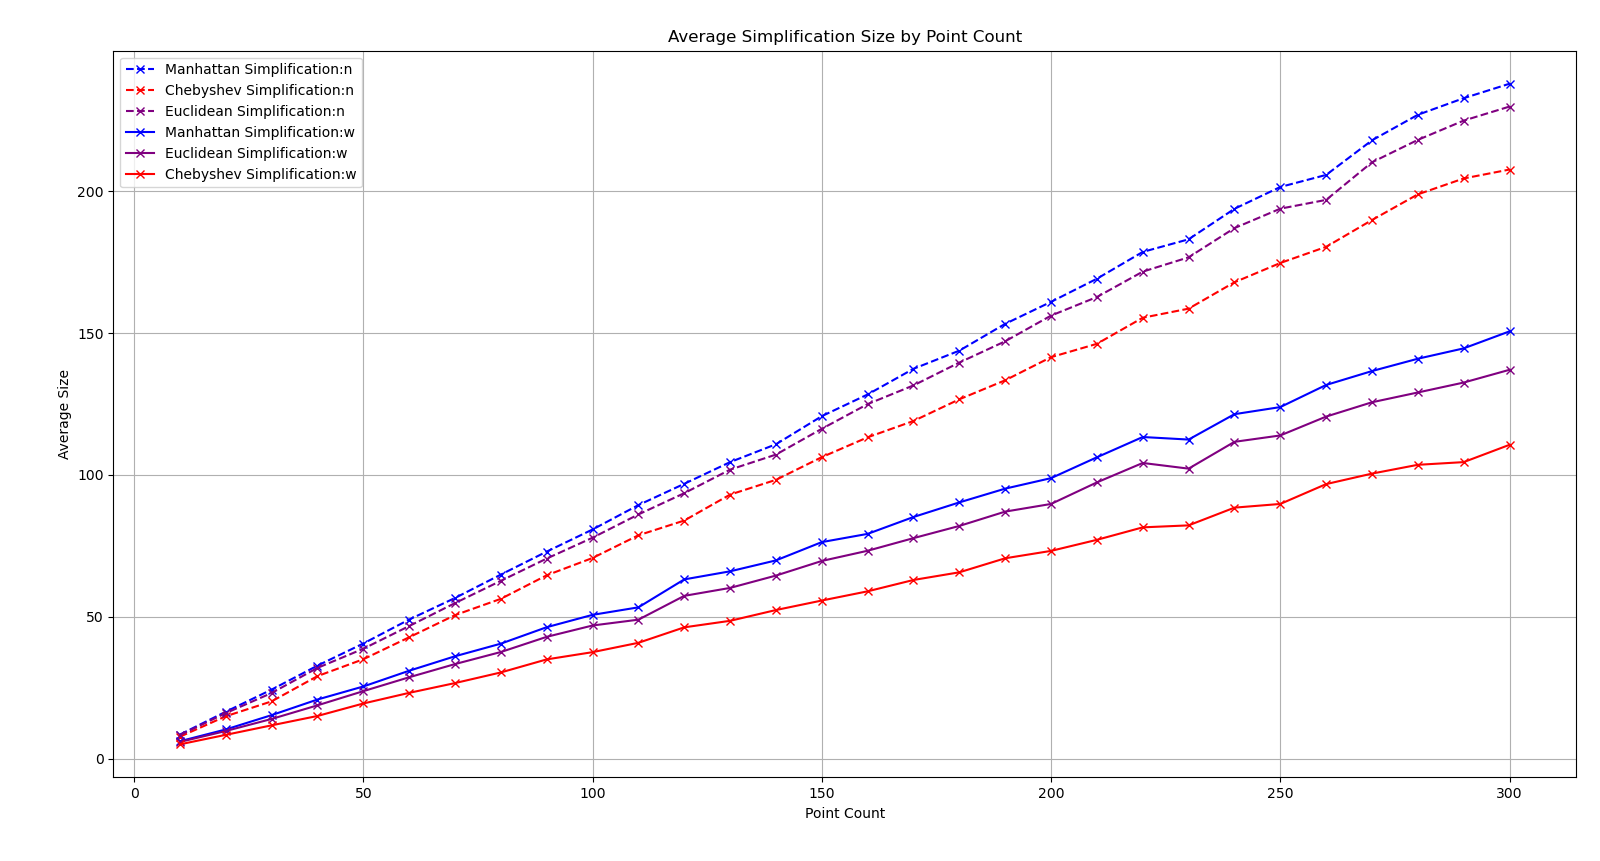
\includegraphics[scale=0.4]{./figures/simplification_sizes.png}
  \caption{Average simplification sizes of the tested data.}
  \label{fig:simplification_sizes}
\end{figure}

Now we investigate the effect of the \(\varepsilon\) on the simplification size in \cref{fig:vary_e10} and \cref{fig:vary_e200}. For this we computed all intervals and the resulting simplification sizes using the algorithm from \cref{sec:simplification-queries}. After the computation, we normalized the \(\varepsilon\) to fit into the interval \([0, 1]\) by dividing by \(\delta(P, e)\) for each polyline \(P\) where \(e\) is the line segment from the first to the last point, i.e., the shortest simplification. Thus for normalized \(\varepsilon > 1\) the plot would be a constant \(2\) is thus not shown. 

Again, we can clearly see a difference between well-behaved and non-well-behaved polylines. Both roughly look like rectangular hyperbolas where the well-behaved data is noticeably closer to the axes which means that a smaller \(\varepsilon\) suffices for a large point reduction. Further, the non-well-behaved data looks less smooth which is possibly because of the greater variance in the data.

Interestingly, all four plots seem to approach concave functions for which we have no explanation.

\begin{figure}[b]
  \centering
	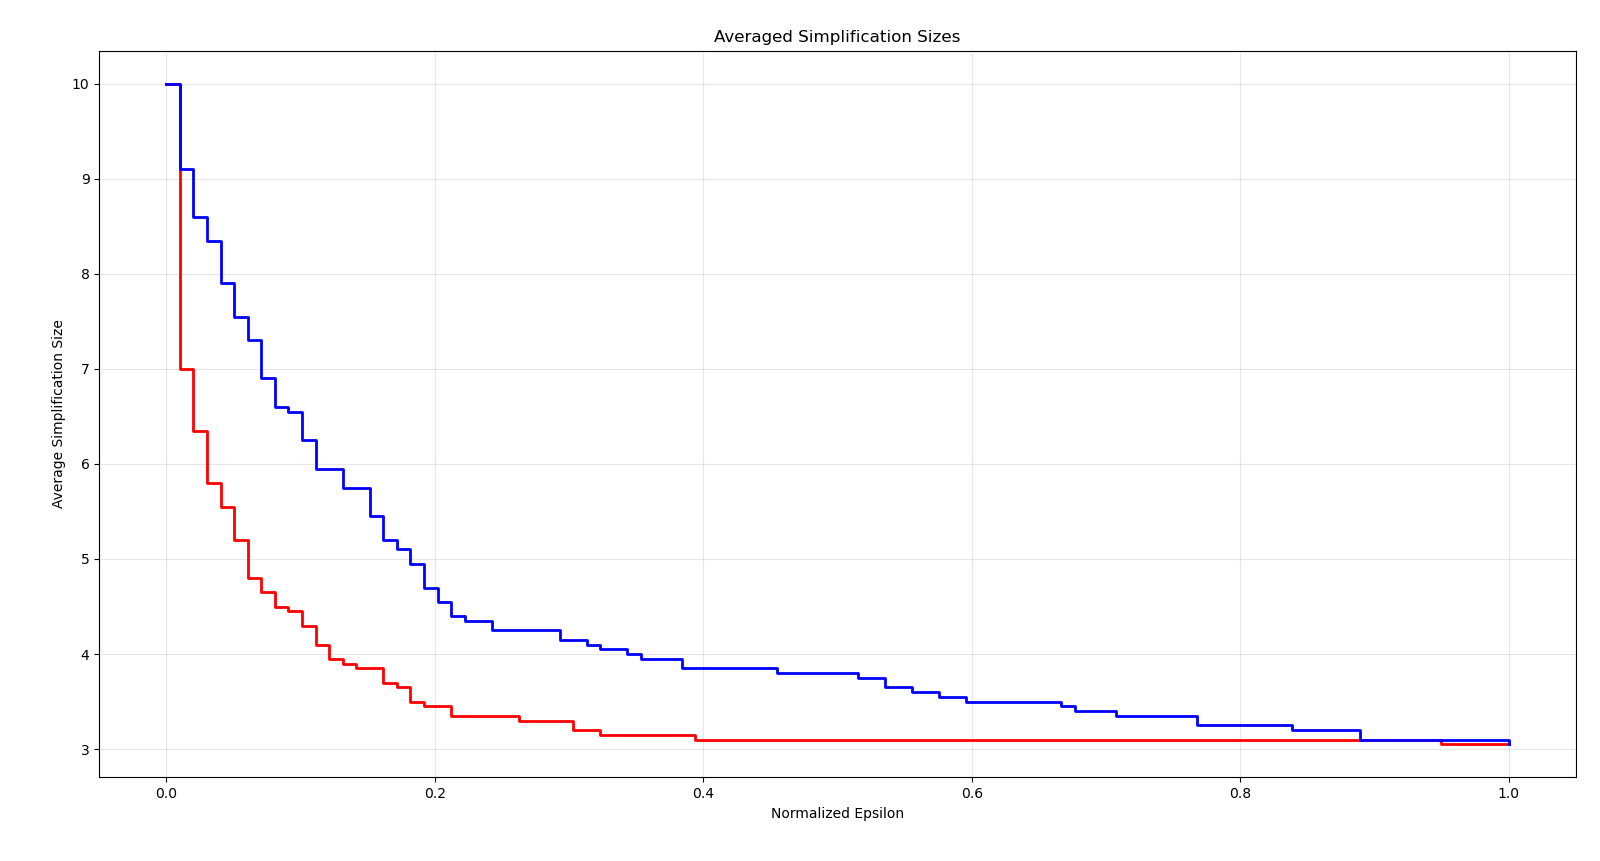
\includegraphics[scale=0.4]{./figures/vary_e10.png}
  \caption{Average simplification sizes of 20 polylines of length 10 over normalized \(\varepsilon\). Well-behaved in red and non-well-behaved in blue.}
  \label{fig:vary_e10}
\end{figure}

\begin{figure}[b]
  \centering
	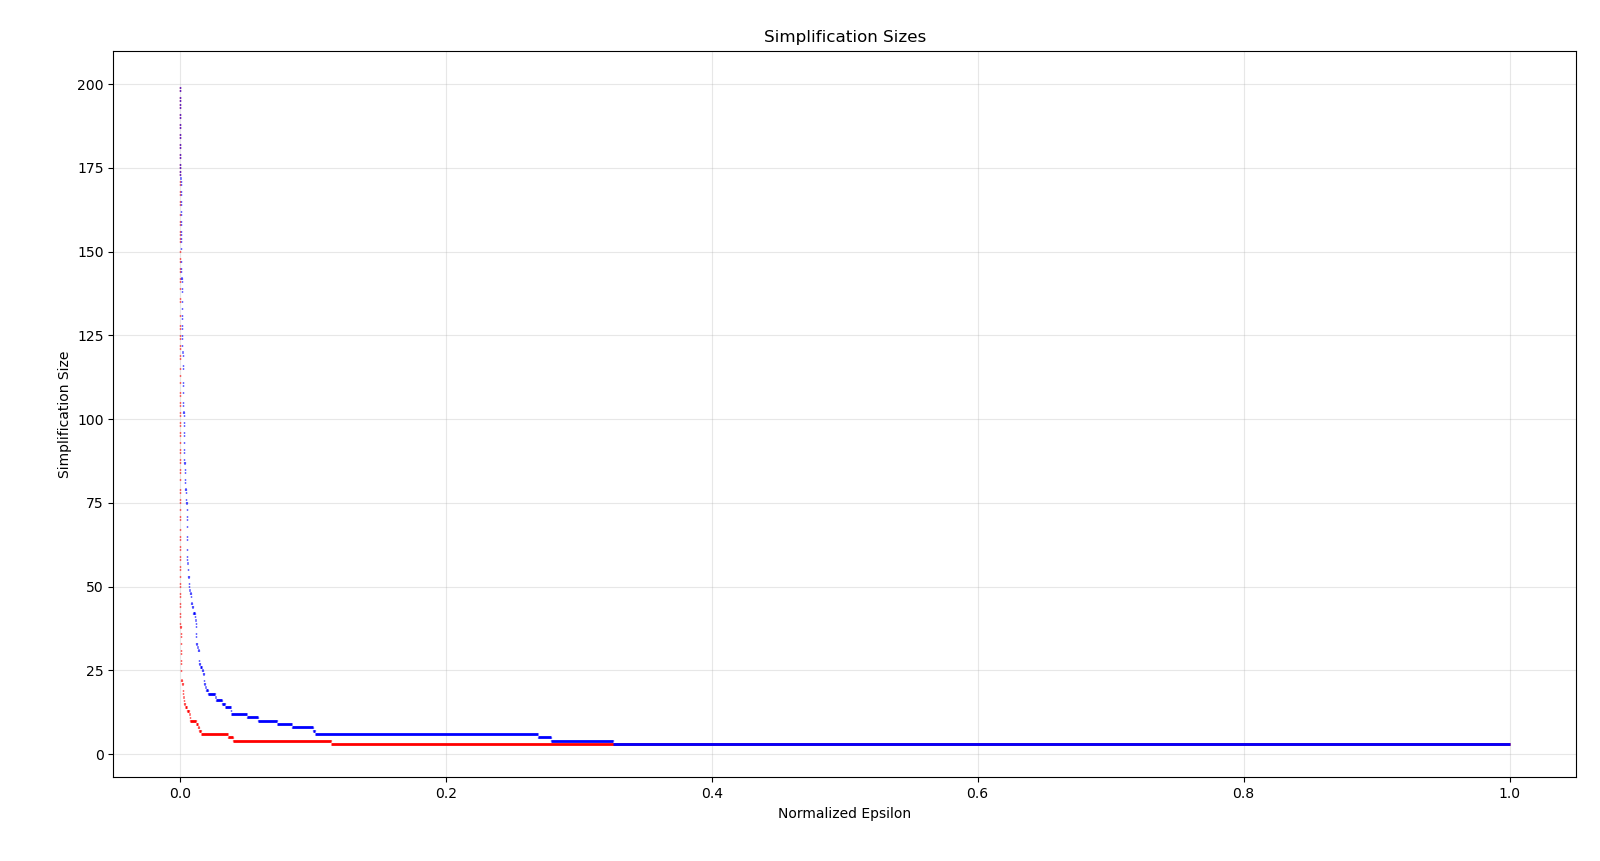
\includegraphics[scale=0.4]{./figures/vary_e200.png}
  \caption{Simplification sizes of a polyline of length 200 over normalized \(\varepsilon\). Well-behaved in red and non-well-behaved in blue.}
  \label{fig:vary_e200}
\end{figure}

Finally, we investigate how local and global simplification sizes differs in \cref{fig:res-local-global}. For this we used the Euclidean variant of the Imai-Iri algorithm to compare against and plot the average simplification sizes on well-behaved and non-well-behaved data. This might be the most surprising result as the sizes do not differ in any meaningful way. On well-behaved data they are indistinguishable and on non-well-behaved the local simplifications are marginally larger.

\begin{figure}[b]
  \centering
	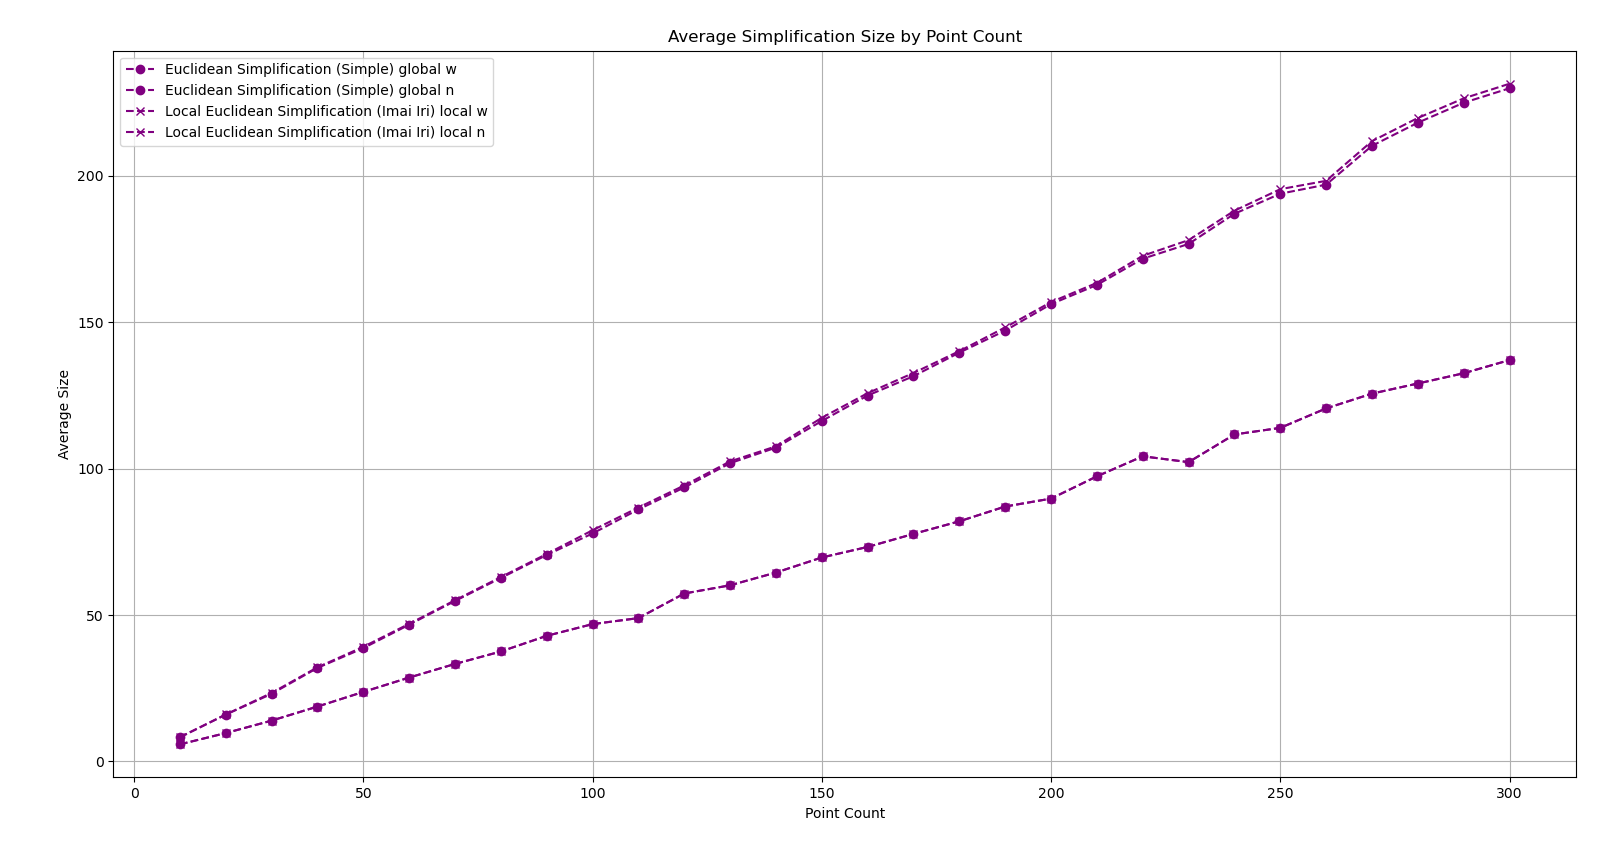
\includegraphics[scale=0.4]{./figures/res_local_global.png}
  \caption{Comparison of local and global simplification sizes on well-behaved and non-well-behaved data.}
  \label{fig:res-local-global}
\end{figure}

Seeing this, we tried varying all parameters of our data generation method to try to find polylines and a suitable \(\varepsilon\) where the local and global distances have a large difference. For this, we chose random values for the minimum and maximum line segment length, and the maximum angle. All polylines tested had a point count of \(150\) and were two dimensional. For each configuration, we automatically tested 1000 polylines with a randomly generated \(\varepsilon\). The highest difference we encountered was \(8\) and the average difference over the \(1000\) iterations was never more than \(0.3\), meaning that on average there is no difference. This suggests that the global and local Fréchet distance are for all practical purposes the same and differ only in degenerate, artificially crafted counterexamples.
